\documentclass[fleqn,letterpaper,12pt]{article}

\usepackage[document]{ragged2e}
\usepackage{times,mathptmx,helvet}
\usepackage{graphicx} % use \usepackage[demo]{graphicx} to suppress figures
% \usepackage{pdfsync}
\usepackage{amsmath}
\usepackage[sort&compress]{natbib}
\setcitestyle{square} % this might be needed

% The lineno packages adds line numbers. Start line numbering with
% \begin{linenumbers}, end it with \end{linenumbers}. Or switch it on
% for the whole article with \linenumbers.
\usepackage{lineno}

\usepackage{enumitem}
\setlist{nosep,labelsep=1.25em,itemindent=.75em}

\usepackage{siunitx}
\sisetup{
    detect-all = true,
    input-decimal-markers = {.},
    input-ignore = {,},
    inter-unit-product = \ensuremath{{}\cdot{}},
    multi-part-units = repeat,
    number-unit-product = \text{~},
    per-mode = fraction,
    separate-uncertainty = true,
}

\usepackage[justification=centering,labelsep=period,figurename=Fig.]{caption}
\captionsetup[table]{justification=raggedright, singlelinecheck=off}

\usepackage{url}
\usepackage{hyperref}
\usepackage{titlesec}

\titleformat{\section}{\normalfont\fontsize{12}{15}\bfseries}{\thesection.}{0.5em}{}
\titleformat{\subsection}{\normalfont\fontsize{12}{15}\bfseries}{\thesubsection}{0.5em}{}
\titleformat{\subsubsection}{\normalfont\fontsize{12}{15}\bfseries}{\thesubsubsection}{0.5em}{}

\titlespacing*{\section}{0pt}{\parskip}{0pt}
\titlespacing*{\subsection}{0pt}{\parskip}{0pt}
\titlespacing*{\subsubsection}{0pt}{\parskip}{0pt}
\titlespacing*{\paragraph}{0pt}{\parskip}{5pt}

\hypersetup{colorlinks=true, urlcolor=blue, citecolor=black, linkcolor=black}
\urlstyle{same}

\setlength{\paperwidth}{8.5in}
\setlength{\paperheight}{11.0in}
\setlength{\textwidth}{6.5in}
\setlength{\textheight}{9in}
\setlength{\topmargin}{0in}
\setlength{\headheight}{0in}
\setlength{\headsep}{0in}
\setlength{\parindent}{0in}
\setlength{\parskip}{\baselineskip}
\setlength{\footskip}{0.25in}
\setlength{\oddsidemargin}{0in}
\setlength{\evensidemargin}{0in}
\setlength{\mathindent}{0cm}
\setlength{\topsep}{0cm}
\setlength{\labelsep}{.8cm}



\begin{document}

\linenumbers

% \bibliographystyle{unsrtnat}
% \setcitestyle{numbers,citesep={,\!}} % cite style is [1,2] instead of [1, 2] (remove space)

\begin{flushleft}
\textbf{Formatting your paper for the 14th International Symposium on Fire Safety Science}\\
\vspace{8pt}
Jane Doe$^{\mathrm{a},*}$, John Q.~Public$^\mathrm{b}$\\
\vspace{8pt}
$^\mathrm{a}$University of Someplace, 1234 Lucky Ln, Someplace, USA, jdoe@usomeplace.edu \\
\vspace{8pt}
$^\mathrm{b}$University of Someplace, 1234 Easy St, Someplace, Canada, jqpublic@usomeplace.edu \\
\vspace{8pt}
$^*$Corresponding author
\end{flushleft}
\rm

\section*{Highlights:}

\begin{itemize}
\item Three to five bullet points
\item Each have maximum 85 characters including spaces
\item Cover main findings
\item Usually submitted separately
\end{itemize}

\section*{Abstract:}

This template should provide the necessary formatting information for submissions to the 14th International Symposium on Fire Safety Science (IAFSS 2023).  The abstract should be concise and factual.  It should contain brief statements on the purpose, results, and major conclusions of the research and should stand alone.  The abstract should be 200 words or less.

\paragraph*{Keywords:} fire chemistry; modeling; suppression

Please provide no more than 10 keywords.  Suggested Keywords: fire chemistry; modeling; human behavior; risk assessment; performance-based design; statistics; structural response; structural design; suppression; detection; forensics; smoke management; flame spread; fire growth; compartment fires; heat transfer; fluid dynamics; CFD; wildfires; explosion; ignition; smoke; toxicity; self-heating; heat release rate; human factors; response patterns; egress; hazard evaluation; reliability; compartmentalization; protection of steel; protection of concrete; protection of wood; fire investigation; transportation fires; industrial fires.

\section{Introduction}

This template should provide the necessary formatting information for submissions to the 14th International Symposium on Fire Safety Science (IAFSS 2023).  The proceedings will be published as a special issue of Fire Safety Journal.  If any questions arise, please consult the requirements and information listed by Fire Safety Journal \cite{Example}.  In general, the formatting of the paper should be as simple as possible.  For example, using the text justification feature of MS Word is unnecessary.  Please use size 12 Times New Roman font.  Margins should be set to 2.5 cm (1 in) for all sides.  Spacing after paragraphs should be 8pt and all text single spaced.

The paper should be divided into numbered sections, as is done here.  Some papers may include other sections not listed here, such as one providing details on theory or thorough discussion of the results.  If subsections are necessary, please number them as indicated in the results section below.

Write out abbreviations or acronyms at their first mention in the text followed by the abbreviation or acronym in parenthesis.  Symbols must be defined either in the text or in a Nomenclature Listing table.  Symbol definitions should include the units of the symbol.  Please use the international system of units (SI).

References should be cited in the text as numbers in square brackets, such as \cite{Example}, in the order in which they appear.  Please make sure that all references made in the text appear in the list at the end of the paper and vice versa.  No specific format of the references is required, but please be consistent.  The use of DOI in references is encouraged. \nocite{Drysdale:1,Magnussen:1,SFPE:Beyler,Rehm:1}

Submitted papers should be no more than \textbf{16 pages maximum} (not including separate figure caption list).  Submissions longer than this will not be considered.

\section{Materials and Methods}

This section should provide enough details that the work can be reproduced by an outside researcher.  

\section{Results}

Please present the results clearly and concisely.

\subsection{Formatting for figures}

Please include the figures in the text where and how they are intended to be viewed (correct size and approximate location).  After the review process is completed and provided that your paper is accepted, the last step before publication will also require that you submit figures as separate files.  All figures should be consecutively numbered and have captions.  Please list all figures captions separately at the end of the text as indicated below.  Detailed instructions on image quality and other requirements are provided in the Guide for Authors for the Fire Safety Journal \cite{Example}.  Note that all figures in the online version will be in color at no additional cost.  If color in the print version is desired, please clearly indicate this upon submission.  Elsevier will send cost information after acceptance.  A sample figure appears in Fig.~\ref{fig_pyrolysis_model}.

\begin{figure}[h!]
\centering
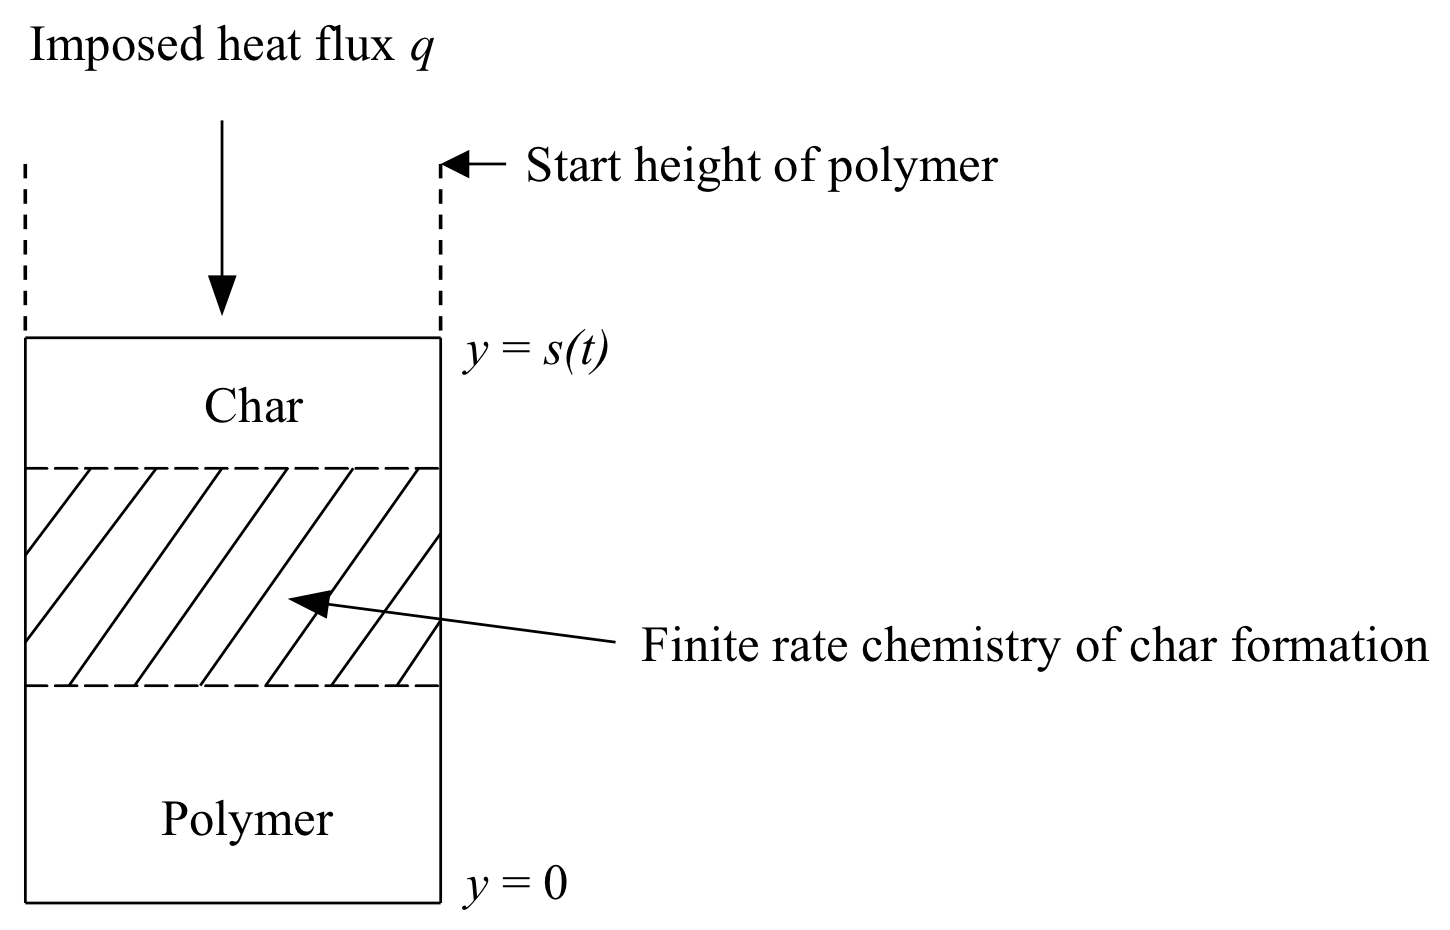
\includegraphics[width=.5\linewidth]{iafss_fig1.png}
\vskip-.2cm
\caption{Figure captions should concisely describe the image.}
\label{fig_pyrolysis_model}
\end{figure}

\subsection{Formatting for tables}

Tables should be inserted as editable text, not as figures.  Tables should also be placed in the text at the appropriate location.  Number tables consecutively and place table notes directly below the table.  Each table should also have a caption.  Please try to avoid using vertical rules and shading. A sample table appears in Table \ref{example_table}.

\begin{table}[h!]
\begin{minipage}{.9\textwidth}
\renewcommand*\footnoterule{}
\renewcommand{\thefootnote}{\alph{footnote}}
\renewcommand*{\arraystretch}{1.4}
\caption{Table captions should concisely describe the content in the table.}
\small
\begin{tabular}{|l|r|r|}
\hline
{\bf Sample type}  & {\bf Time to ignition}  & {\bf Critical heat flux for ignition} \\
                   & {\bf[s]}            & {\bf [\si{kW/m^2}]} \\ \hline   
Sample A           & 140 ($\pm$9)   &  25 ($\pm$1.1)  \\ \hline
Sample B           & 283 ($\pm$16)  &  28 ($\pm$1.5)  \\ \hline
Sample C           & 316 ($\pm$5)   &  29 ($\pm$1.2)  \\ \hline
\end{tabular}
\label{example_table}
\end{minipage}
\end{table}

\subsection{Formatting for equations}

Equations should be inserted as editable text, not as figures.  Simple equations can be in line with normal text.  Ratios should be indicated with the “/” symbol such as As/V.  When not in line with text, please consecutively number all equations.  An example equation is shown in Eq.~(\ref{eq_quadratic_formula}).
\begin{equation}
\label{eq_quadratic_formula}
x = \frac{-b \pm \sqrt{b^2-4ac}}{2a}
\end{equation}

\section{Conclusions}

The main conclusions of the study may be summarized here.

\section*{Acknowledgements}

Acknowledgements from the authors can be listed here.  Please list grant numbers when listing funding sources.

\bibliographystyle{elsarticle-num}
\bibliography{References}

\end{document}
